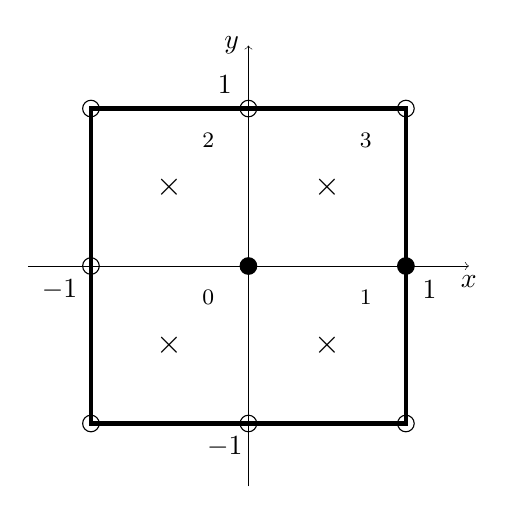
\begin{tikzpicture}[scale=2.0]
% axes
  \draw[->,very thin] (-1.4,0.0) -- (1.4,0.0) node[below] {$x$};
  \draw[->,very thin] (0.0,-1.4) -- (0.0,1.4) node[left] {$y$};
  \node at (1.15,-0.15) {$1$};
  \node at (-1.2,-0.15) {$-1$};
  \node at (-0.15,1.15) {$1$};
  \node at (-0.15,-1.15) {$-1$};
% domain and elements
  \draw[line width=1.5pt] (-1,-1) -- (1,-1) -- (1,1) -- (-1,1) -- cycle;
  \node at (-0.25,-0.2) {\large $\square_0$};
  \node at (0.75,-0.2) {\large $\square_1$};
  \node at (-0.25,0.8) {\large $\square_2$};
  \node at (0.75,0.8) {\large $\square_3$};
% velocity unknowns
  \filldraw (0.0,0.0) circle (1.5pt);
  \filldraw (1.0,0.0) circle (1.5pt);
% Dirichlet nodes
  \draw (-1.0,-1.0) circle (1.5pt);
  \draw (-1.0,0.0) circle (1.5pt);
  \draw (-1.0,1.0) circle (1.5pt);
  \draw (0.0,-1.0) circle (1.5pt);
  \draw (0.0,1.0) circle (1.5pt);
  \draw (1.0,-1.0) circle (1.5pt);
  \draw (1.0,1.0) circle (1.5pt);
% pressure unknowns
  \node at (-0.5,-0.5) {\large $\times$};
  \node at (-0.5,0.5) {\large $\times$};
  \node at (0.5,-0.5) {\large $\times$};
  \node at (0.5,0.5) {\large $\times$};
\end{tikzpicture}

